\documentclass[12pt,a4paper]{article}
\usepackage{amsmath,amsfonts,amssymb}
\usepackage{graphicx}
\usepackage{enumitem}
\usepackage[dvipsnames]{xcolor}
\usepackage{pgfplots}
\usepackage{hyperref}
\usepackage{soul}
\usepackage{framed}
\usepackage{booktabs} 
\usepackage{tabularx}
\usepackage{array}
\usepackage{adjustbox}
\usepackage{siunitx}
\usepackage{subcaption}
\usepackage{tikz}
\usepackage{float}
\pgfplotsset{width=10cm ,compat=1.9}


\renewcommand{\arraystretch}{1.5}
\setlength{\tabcolsep}{12pt}

\newlist{arrowlist}{itemize}{1}
\setlist[arrowlist]{label=$\Rightarrow$}

\definecolor{lessonbgcolor}{rgb}{0.9,0.9,1}
\definecolor{examplecolor}{rgb}{0.8,1,0.8}
\definecolor{noteboxcolor}{rgb}{1,0.8,0.8}
\newenvironment{lesson}[1]
  {\begin{framed}\colorbox{lessonbgcolor}{
  \parbox{\dimexpr\linewidth-2\fboxsep}{
  \textbf{#1}}}\end{framed}}
  
\newenvironment{example}
  {\begin{framed}\colorbox{examplecolor}{
  \parbox{\dimexpr\linewidth-2\fboxsep}{
  \textbf{Example:}}}}
  {\end{framed}}
\newenvironment{note}
  {\begin{framed}\colorbox{noteboxcolor}{
  \parbox{\dimexpr\linewidth-2\fboxsep}{
  \textbf{Note:}}}}
  {\end{framed}}

\usepackage{mathtools}
\usepackage[
  amsmath
]{empheq}
\usepackage{xcolor}

\definecolor{shadecolor}{cmyk}{0,0,0.45,0}
\definecolor{light-blue}{cmyk}{0.25,0,0,0}
\newsavebox{\mysaveboxM}
\newsavebox{\mysaveboxT}
\newcommand*\Garybox[2][Log law]{%
  \sbox{\mysaveboxM}{#2}%
  \sbox{\mysaveboxT}{\fcolorbox{black}{light-blue}{#1}}%
  \sbox{\mysaveboxM}{%
    \parbox[b][\ht\mysaveboxM+0.5\ht\mysaveboxT+0.5\dp\mysaveboxT][b]{%
      \wd\mysaveboxM}{#2}%
  }%
  \sbox{\mysaveboxM}{%
    \fcolorbox{black}{shadecolor}{%
      \makebox[\linewidth-17.5em]{\usebox{\mysaveboxM}}%
    }%
  }%
  \usebox{\mysaveboxM}%
  \makebox[0pt][r]{%
    \makebox[\wd\mysaveboxM][c]{%
      \raisebox{\ht\mysaveboxM-0.5\ht\mysaveboxT
                +0.5\dp\mysaveboxT-0.5\fboxrule}{\usebox{\mysaveboxT}}%
    }%
  }%
}
  

\pgfplotsset{width=7cm,compat=1.17}
\begin{document}
\section*{Unit 4: Exponential Functions}
 
\section*{Radicals}
\begin{lesson}{Parts of radicals}

$$\sqrt[n]{a}$$    
\begin{enumerate}
\item \textcolor{blue}{n = index or root}
\item \textcolor{blue}{a = Radicand}
\end{enumerate}
\end{lesson}

\begin{lesson}{PROPERTIES OF RADICALS }
\begin{enumerate}
    \item A. $a^{\frac{1}{n}}=\sqrt[n]{a}$
    \item B. $a^{\frac{m}{n}}=\sqrt[n]{a}=(\sqrt[n]{a})^m$
    \item C. $\sqrt[n]{a^n} = a^{\frac{n}{n}}$
    \item D. $\sqrt[n]{ab} \cdot \sqrt[n]{b}$
\end{enumerate}
\end{lesson}

\begin{example}
\begin{enumerate}
    \item $x^{\frac{1}{3}} = \sqrt[3]{x}$ 
    \item $x^{\frac{2}{3}}= \sqrt[3]{x^2}$ or $(\sqrt[3]{x})^2$
    \item $\sqrt{x^2} = x$ \quad $\sqrt[5]{x^5}=x$
\end{enumerate}    
\end{example}
\newpage
\begin{example}
\begin{enumerate}
    \item 1. $\sqrt{36y^4} = \sqrt{36} \cdot \sqrt{y^4}=6y^2$
    \item 2. $\sqrt{72y^5}= \sqrt{36y^4} \cdot \sqrt{2y}= 6y^2 \sqrt{2y}$
    \item 3. $\sqrt[3]{48y^7}= \sqrt[3]{8y^6} \cdot \sqrt[3]{6y}=2y^2 \sqrt[3]{6y}$
    \item 4. $\sqrt[4]{64x^5 y^8}= \sqrt[4]{16x^4y^8} \sqrt[4]{4x}=2xy^2 \sqrt[4]{4x}$
    \item 5. $\sqrt[5]{64x^5y^8} = \sqrt[5]{32x^5y^5} \cdot \sqrt[5]{2y^5}=2xy^5 \sqrt{2y^5}$
    \item 6. $\sqrt{\frac{9}{16}}= \frac{\sqrt{9}}{\sqrt{16}} =\frac{3}{4}$
    \item 7. $\sqrt[3]{\frac{8y^4}{27x^3}}=\frac{\sqrt[3]{8y^4}}{\sqrt[3]{27x^3}}=\frac{\sqrt[3]{8y^3} \cdot \sqrt[3]{y}}{\sqrt[3]{27x^3}}= \frac{2y^3 \sqrt{y}}{3x}$
    \item 8. $\sqrt{\frac{x^2}{4y^2}}= \frac{\sqrt{x^2}}{\sqrt{4y^2}}= \frac{x}{2y}$
\end{enumerate}
\end{example}
\newpage
\begin{lesson}{Rationalizing the Denominator}
When simplifying fractions with radicals, you need to rationalize the denominator by multiplying the numerator and the denominator by the \textbf{smallest value that will allow you to eliminate the the radical in the denominator}, as shown below. 
\end{lesson}
\begin{example}
\begin{enumerate}
    \item 1. $\sqrt{\frac{1}{5}}= \frac{\sqrt{1}}{\sqrt{5}}= \frac{1}{\sqrt{5}}\cdot \textcolor{red}{\frac{\sqrt{5}}{\sqrt{5}}}=\frac{\sqrt{5}}{\sqrt{25}}=\frac{\sqrt{5}}{5}$
    \item 2. $\sqrt{\frac{2}{3}}= \frac{\sqrt{2}}{\sqrt{3}} \cdot \textcolor{red}{\frac{\sqrt{3}}{\sqrt{3}}} = \frac{\sqrt{6}}{3}$ 
    \item 3. $\sqrt[3]{\frac{1}{x}} = \frac{\sqrt[3]{1}}{\sqrt[3]{x}}= \frac{1}{\sqrt[3]{x}} \cdot \textcolor{red}{\frac{\sqrt[3]{x^2}}{\sqrt[3]{x^2}}}= \frac{\sqrt[3]{x^2}}{\sqrt[3]{x^3}}= \frac{\sqrt[3]{x^2}}{x}$
    \item 4. $\sqrt[4]{\frac{4p^8}{8p^8}}= \sqrt[4]{\frac{p^2}{2}}= \frac{\sqrt[4]{p^2}}{\sqrt[4]{2}} \cdot \textcolor{red}{\frac{\sqrt[4]{2^3}}{\sqrt[4]{2^3}}}=\frac{\sqrt[4]{8p^2}}{2}$
\end{enumerate}    
\end{example}
\begin{note}
Rules for Simplifying Radicals:
\begin{enumerate}
\item There should be no factor in the radicand that has a power greater than or equal to the index.
\item There should be no fractions under the radical sign.
\item There should be no radicals in the denominator (i.e. the denominator should be rationalized).
\end{enumerate}
\end{note}
\newpage 
\begin{lesson}{ADDITION AND SUBTRACTION}

    Radicals may be added or subtracted when they have the same index \underline{and} the same radicand(just like combining like terms).
\begin{note}
    When adding or subtracting radicals, the index and radicand do \underline{not} change.
\end{note}    
\end{lesson}
\begin{example}
\begin{enumerate}
    \item a. $5\sqrt{2}-8\sqrt{2}=-3\sqrt{2}$
    \item b. $6x\sqrt[3]{3}+2x\sqrt[3]{3}= 8x\sqrt[3]{3}$
    \item c. $5\sqrt[5]{xy}+6\sqrt[5]{xy}= 11\sqrt[5]{xy}$
    \item d. $7\sqrt{x} - 9\sqrt[3]{x} +4\sqrt[3]{x}= 7 \sqrt{x} - 5\sqrt[3]{x}$
    \item e. $\sqrt{75}+2\sqrt{12}-5\sqrt{3}=\sqrt{25}\sqrt{3}+2\sqrt{4}\sqrt{3}-5\sqrt{3}+4\sqrt{3}-5\sqrt{5}=4\sqrt{3}$
\end{enumerate}    
\end{example}
\newpage
\begin{lesson}{MULTIPLICATION OF RADICALS}
    To multiple radicals, just multiply using the same rules as multiplying polynomials (Distributive Property, FOIL, and Exponent Rules) except \textbf{NEVER} multiply values outside of the radicals times values inside the radical.
\end{lesson}
\begin{example}
\begin{enumerate}
    \item a. $\sqrt{20x^3} \cdot \sqrt{4xy^6}= \sqrt{80x^4y^7}=\sqrt{16x^4y^6} \cdot \sqrt{5y} = 4x^2y^3\sqrt{5y}$
    \item b. $2x\sqrt{3xy} \cdot 4\sqrt{2x^5y}$
    \item c. $2\sqrt{5}(3\sqrt{2}-\sqrt{5})=6\sqrt{10}-2\sqrt{25}=  6\sqrt{10}-10$
    \item d. $(2\sqrt{x}+2)(\sqrt{x}+3)=2\sqrt{x^2}+6\sqrt{x}+2\sqrt{x}+6$
\end{enumerate}    
\end{example}
\begin{note}
When multiplying radicals with different indexes, change to rational exponents first, find a common denominator in order to add the exponents, then rewrite in radical notation as shown below: \\
Example: $\sqrt[3]{x^2} \cdot \sqrt[6]{x^5}=x^{\frac{2}{3}} \cdot x^{\frac{5}{6}}= x^{\frac{4}{6}}\cdot x^{\frac{5}{6}}= x^{\frac{3}{2}}=\sqrt{x^3}=\sqrt{x^2}\sqrt{x}=x\sqrt{x}$
\end{note}
\newpage
\begin{lesson}{MORE RATIONALIZING THE DENOMINATOR: (DIVISION)}
    If the denominator contain two terms such that at least one term has a radical, multiply the numerator and the denominator by the \textbf{conjugate} of the denominator:
    \textbf{Conjugate} - the conjugate of a binomial of the form (a+b) is (a-b).
    Example: The conjugate of $(\sqrt{x}-3) is (\sqrt{x}+3).$
\end{lesson}
\begin{note}
    Since $(a+b)(a-b)=a^2-b^2$, eliminating the middle term, multiplying by the conjugate eliminates the middle term that would still have a radical in it, thus removing the radical from the denominator.
\end{note}
\begin{example}
\begin{align*}
    &a. \frac{1}{\sqrt{x}+1} \cdot \frac{\sqrt{x}-1}{\sqrt{x}-1} = \frac{\sqrt{x}-1}{\sqrt{x^2}-1} = \frac{\sqrt{x}-1}{x-1} \\
    &b. \frac{6}{\sqrt{5}-\sqrt{2}} \cdot \frac{\sqrt{5}+\sqrt{2}}{\sqrt{5}+\sqrt{2}} = \frac{6(\sqrt{5}+\sqrt{2})}{5-2} = \frac{6(\sqrt{5}+\sqrt{2})}{3} = 2(\sqrt{5}+\sqrt{2})
\end{align*}
\end{example}
\newpage
\section*{Exponent Laws}
\begin{lesson}{Exponent Laws}
 
\subsection*{Product Law}
When multiplying two terms with the same base, add the exponents.
\[ a^m \cdot a^n = a^{m + n} \]

\subsection*{Quotient Law}
When dividing two terms with the same base, subtract the exponents.
\[ \frac{a^m}{a^n} = a^{m - n} \]

\subsection*{Power Law}
When raising a power to another power, multiply the exponents.
\[ (a^m)^n = a^{mn} \]

\subsection*{Zero Exponent Law}
Any nonzero number raised to the power of zero is equal to 1.
\[ a^0 = 1 \]

\subsection*{Negative Exponent Law}
\[ a^{-n} = \frac{1}{a^n} \]
\subsection*{Exponent Laws}
\begin{enumerate}[label=\arabic*.]
    \item \( x^3 \cdot x^4 = x^{3 + 4} = x^7 \)
    \item \( \frac{y^6}{y^3} = y^{6 - 3} = y^3 \)
    \item \( a^5 \cdot a^{-2} = a^{5 - 2} = a^3 \)
    \item \( \frac{b^8}{b^4} = b^{8 - 4} = b^4 \)
\end{enumerate}
\newpage
\section*{Logarithms}
\begin{lesson}{Logarithms}
\subsection*{Introduction to Logarithms}
Logarithms are the inverse operations of exponentiation.

\subsection*{Properties of Logarithms}
\begin{enumerate}[label=\alph*.]
    \item \( \log_b(a \cdot c) = \log_b(a) + \log_b(c) \)
    \item \( \log_b\left(\frac{a}{c}\right) = \log_b(a) - \log_b(c) \)
    \item \( \log_b(a^n) = n \cdot \log_b(a) \)
\end{enumerate}

\subsection*{Common Logarithm and Natural Logarithm}
\begin{enumerate}[label=\alph*.]
    \item Common logarithm: \( \log_{10}(x) = \log(x) \)
    \item Natural logarithm: \( \ln(x) \)
\end{enumerate}
\end{lesson}
\section*{Examples}
\subsection*{Logarithms}
\begin{enumerate}[label=\arabic*.]
    \item \( 10^x = 100 \) implies \( x = 2 \)
    \item \( \log_2(8) = 3 \) because \( 2^3 = 8 \)
    \item \( e^y = 20 \) implies \( y = \ln(20) \)
    \item \( \ln(1) = 0 \) because \( e^0 = 1 \)
\end{enumerate}
\end{lesson}
\newpage 
\begin{lesson}{Solving equations with logarithms}
\begin{arrowlist}
 \item The logarithms of a \# to given base is the exponent that must be used with that base to obtain the given \#.
 \begin{example}
     The logarithms of $64$ to base $2$ is $6$ since $2^6 = 64$
 \end{example}
 We would write that as: $\log_2 64 = 6$.
 \begin{itemize}
     \item $\log_2$ - base.
     \item $64$ - argument.
     \item $6$ - logarithms.
 \end{itemize}

\item The logarithm function is the $\underbrace{\textbf{\textcolor{blue}{inverse}}}_{\text{(Switch $x$ and $y$)}}$ function of an exponent.

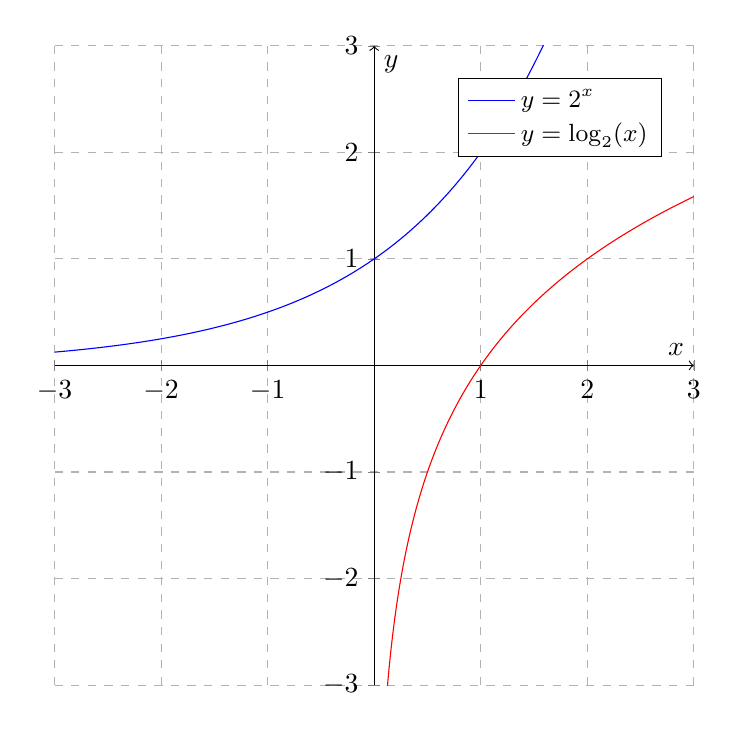
\begin{tikzpicture}
    \begin{axis}[
        xlabel=$x$,
        ylabel=$y$,
        xmin=-3, xmax=3,
        ymin=-3, ymax=3,
        axis lines=middle,
        axis line style={->},
        legend style={at={(0.95,0.95)},anchor=north east},
        grid=both,
        major grid style={dashed,gray!60},
        width=0.8\textwidth,
        height=0.8\textwidth,
        legend style={font=\small},
        legend cell align={left},
    ]
    
    % Plot y=2^x
    \addplot[blue, domain=-3:2, samples=100, smooth] {2^x};
    \addlegendentry{$y = 2^x$}
    
    % Plot y=log_2(x)
    \addplot[red, domain=0.1:3, samples=100, smooth] {log2(x)};
    \addlegendentry{$y = \log_2(x)$}
    
    \end{axis}
\end{tikzpicture}
\end{arrowlist}

\newpage
\begin{arrowlist}
 \item In general we write $y= \log_a x$ where a is the base and x is the argument 
\end{arrowlist}
\end{lesson}
\begin{example}
Determine the logs:
\begin{enumerate}[label=\alph*.]
    \item $\log_{10} 1000= 3$ since $10^3=1000$
    \item $\log_5 625 = 5^x= 625= x=4$
    \item $\log_2 1024= 10$
    \item $\log_b b=1$
    \item $\log_2 1=0$
\end{enumerate}
\end{example}
\begin{example}
Express in exponential form:
    \begin{enumerate}
        \item $m =\log_3 81 \Rightarrow3^m=81$
        \item $y=\log_7 (\frac{1}{7}) \Rightarrow 7^y=\frac{1}{7}$
        \item $n=\log _a n \Rightarrow a^m=n$
    \end{enumerate}
\end{example}
\begin{example}
    Express as logarithm
    \begin{enumerate}
        \item $2^5=32 \Rightarrow 5=\log_2 32$
        \item $3^m=343 \Rightarrow m=\log_3 343$
        \item $\frac{1}{25}= 5^x \Rightarrow n=\log_5 (\frac{1}{25})$
    \end{enumerate}
\end{example}
\newpage
\begin{example}
Use your calculator to Evaluate
    \begin{enumerate}
        \item $\log_6 216 \Rightarrow 3$
        \item $\log_7 117649 \Rightarrow \frac{\log 117649}{\log 7}=6$
        \item $\log 1000000 \Rightarrow$ base 10(common log) $=6$
    \end{enumerate}
\end{example}

\begin{empheq}[box = {\Garybox[Log law]}]{align*}
    1. & \log a^x \Rightarrow x \log a \\
    2. & a^x = (10^{\log a})^x \Rightarrow a^x =10^{x \log a}
\end{empheq}
\begin{example}
    \begin{enumerate}
        \item $12^x=400 \Rightarrow x = \log_12 400= x=\frac{\log 400}{log 12}= x \approx 2.41$
        \item $1.08^x=4.39 \Rightarrow \log 10.8^x = \log 4.39= x=\frac{log 4.39}{1.08}=x \approx 19.22$
        \item $10^{x-3}=500$
        \begin{align*}
        10^{x-3} &= 500 \\
        \Rightarrow \log 10^{x-3} &= \log 500 \\
        (x-3) \log 10 &= \log 500 \\
        x-3 &= \frac{\log 500}{\log 10} \\
        x-3 &= \frac{\log 500}{\log 10} \\
        x &= 3 + \frac{\log 500}{\log 10} \\
        x &\approx 5.70
    \end{align*}
    \end{enumerate}
\end{example}
\newpage
\section*{Transformation of Exponential Function}
\begin{equation*}
    \underbrace{f(x)=a \cdot b ^{k(k-d)}+C}_{\text{base of exponential f\underline{n}}}
\end{equation*}
Exponential functions can be transformed in the same way as $f(x)=a \cdot b ^{k(k-d)}+C$
other function. The graph of can be found by
performing transformations on the graph of y = bx
\begin{example}
    List transformation applied to \(y=2^x\)
    \begin{enumerate}
        \item \(f(x)=3 \cdot 2^x-5\)
        \begin{itemize}
            \item \textcolor{red}{VS by 3}
            \item \textcolor{red}{Parent function \(y=2^x\)}
            \item \textcolor{red}{VT 5 \(\downarrow\)}
        \end{itemize}
        \item \(f(x)=-2^{x-1}+6\)
        \begin{itemize}
            \item \textcolor{red}{RXA}
            \item \textcolor{red}{HT 1 \(\to\)}
            \item \textcolor{red}{VT 6 \(\uparrow\)}
        \end{itemize}
        \item \(f(x)=\frac{1}{2}(2)^{-x+4} -8\)
        \begin{itemize}
            \item \textcolor{red}{VS by 2}
            \item \textcolor{red}{RXA}
            \item \textcolor{red}{HT 4 \(\to\)}
            \item \textcolor{red}{VT 6 \(\uparrow\)}
        \end{itemize}
        \item \(f(x)=-2^{3x-9}+62\)
        \begin{itemize}
            \item \textcolor{red}{RXA}
            \item \textcolor{red}{HS by \(\frac{1}{3}\)}
            \item \textcolor{red}{VT 62 \(\uparrow\)}
        \end{itemize} 
    \end{enumerate}
\end{example}
\newpage
\begin{example}
    List the the transformation applied to \(y=\left(\frac{1}{4}\right)^x\)
    \begin{enumerate}
        \item $f(x)=3 \left( \frac{1}{4}\right)^{x-10}-8$
    \begin{itemize}
    \item \textcolor{red}{VS}
    \item \textcolor{red}{HT 10 \(\to\)}
    \item \textcolor{red}{VT 8 \(\downarrow\)}
    \end{itemize}  
    \item $g(x)=-\left(\frac{1}{4} \right)^{\frac{1}{2}x}+2$
    \begin{itemize}
    \item \textcolor{red}{RXA}
    \item \textcolor{red}{HS by \(2\)}
    \item \textcolor{red}{VT 2 \(\downarrow\)}
    \end{itemize}     
    \item $h(x)=\frac{1}{3}\left(\frac{1}{4}\right)^{-x-6}$
    \begin{itemize}
    \item \textcolor{red}{VS by \(\frac{1}{3}\)}
    \item \textcolor{red}{RYA}
    \item \textcolor{red}{HT 6 \(\gets\)}
    \end{itemize}       
    \item $p(x)=-3\left( \frac{1}{4}\right)^{2x+1}$
    \begin{itemize}
    \item \textcolor{red}{RXA}
    \item \textcolor{red}{VS by 3}
    \item \textcolor{red}{HT by \(\frac{1}{2}\)}
    \item \textcolor{red}{HS by \(\frac{1}{2}\)}
    \end{itemize}    
    \end{enumerate}
\end{example}
\newpage 
For an exponential function, the horizontal asymptote is only affected by vertical translation. So the equation of the H.A will be $y=c$ \\ \\
When the function is: \\ 
\begin{equation*}
f(x)=a\cdot b^{k(x-d)}+C    
\end{equation*}
\begin{example}
    Find the equation of the horizontal asymptote and determine the $y$-intercept (set $x = 0$).
    \begin{enumerate}
        \item $f(x)=2\cdot 3^x -4 \quad $ H.A $= -4 \quad$ y-int is -2
        \item $g(x)=\frac{1}{2}\left(\frac{1}{8} \right)^{-x}+1 \quad $ H.A $=1 \quad$  y-int is $\frac{3}{2}$
    \end{enumerate}
\end{example}
\begin{lesson}{Exponential Functions}
    \begin{arrowlist}
        \item The domain of exponential function is always: $\{x \in \mathbb{R}\}$. 

        \begin{figure}[h]
            \centering
            \begin{subfigure}{0.45\textwidth}
                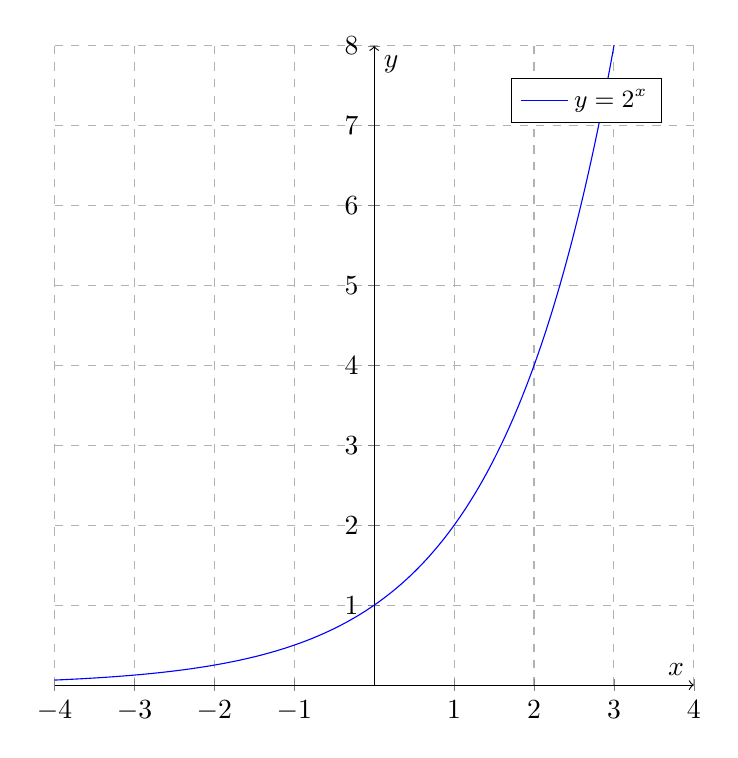
\begin{tikzpicture}
                    \begin{axis}[
                        xlabel=$x$,
                        ylabel=$y$,
                        xmin=-4, xmax=4,
                        ymin=0, ymax=8,
                        axis lines=middle,
                        axis line style={->},
                        legend style={at={(0.95,0.95)},anchor=north east},
                        grid=both,
                        major grid style={dashed,gray!60},
                        width=0.8\textwidth,
                        height=0.8\textwidth,
                        legend style={font=\small},
                        legend cell align={left},
                    ]

                    % Growth function
                    \addplot[blue, domain=-4:4, samples=100, smooth] {2^x};
                    \addlegendentry{$y = 2^x$}

                    \end{axis}
                \end{tikzpicture}
                \caption{Growth}
                \label{fig:growth}
            \end{subfigure}
            %
            \begin{subfigure}{0.45\textwidth}
                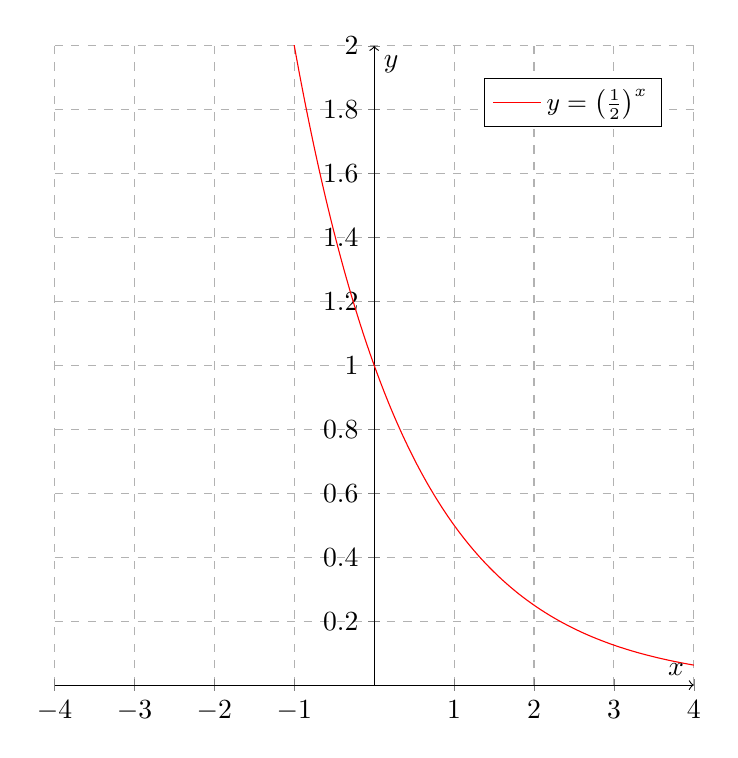
\begin{tikzpicture}
                    \begin{axis}[
                        xlabel=$x$,
                        ylabel=$y$,
                        xmin=-4, xmax=4,
                        ymin=0, ymax=2,
                        axis lines=middle,
                        axis line style={->},
                        legend style={at={(0.95,0.95)},anchor=north east},
                        grid=both,
                        major grid style={dashed,gray!60},
                        width=0.8\textwidth,
                        height=0.8\textwidth,
                        legend style={font=\small},
                        legend cell align={left},
                    ]

                    % Decay function
                    \addplot[red, domain=-4:4, samples=100, smooth] {(1/2)^x};
                    \addlegendentry{$y = \left(\frac{1}{2}\right)^x$}

                    \end{axis}
                \end{tikzpicture}
                \caption{Decay}
                \label{fig:decay}
            \end{subfigure}

            \caption{Growth and Decay}
            \label{fig:growth_decay}
        \end{figure}

        \item The range will depend on the location of the horizontal asymptote and if there was a reflection in the x-axis (RXA).
    \end{arrowlist}
    
% Growth and Decay in 3D plot     
\begin{figure}[H]
    \centering
    \begin{tikzpicture}
        \begin{axis}[
            xlabel=$x$,
            ylabel=$y$,
            zlabel=$z$,
            xmin=-4, xmax=4,
            ymin=0, ymax=8,
            zmin=0, zmax=8,
            axis lines=middle,
            axis line style={->},
            legend style={at={(0.95,0.95)},anchor=north east},
            grid=both,
            major grid style={dashed,gray!60},
            width=0.8\textwidth,
            height=0.8\textwidth,
            legend style={font=\small},
            legend cell align={left},
            view={40}{30}, % Adjust the view angle
            colormap/jet, % Use 'hot' colormap
        ]
            \addplot3[surf,hot,domain=-4:4,domain y=0:8,shader=interp] {2^x};
            \addlegendentry{$z = 2^x$}
        \end{axis}
    \end{tikzpicture}
    \qquad
    \begin{tikzpicture}
        \begin{axis}[
            xlabel=$x$,
            ylabel=$y$,
            zlabel=$z$,
            xmin=-4, xmax=4,
            ymin=0, ymax=8,
            zmin=0, zmax=8,
            axis lines=middle,
            axis line style={->},
            legend style={at={(0.95,0.95)},anchor=north east},
            grid=both,
            major grid style={dashed,gray!60},
            width=0.8\textwidth,
            height=0.8\textwidth,
            legend style={font=\small},
            legend cell align={left},
            view={40}{30}, % Adjust the view angle
            colormap/hot, % Use 'hot' colormap
        ]
            \addplot3[surf,hot,domain=-4:4,domain y=0:8,shader=interp] {(1/2)^x};
            \addlegendentry{$z = \left(\frac{1}{2}\right)^x$}
        \end{axis}
    \end{tikzpicture}
    \caption{Growth and Decay in 3D Plot}
\end{figure}
\end{lesson}
\newpage 


\newpage
\section*{Examples}
\begin{example}
\begin{enumerate}
   \item $f(x) = 2^x + 4$
   
   \begin{minipage}{0.8\textwidth}
       \begin{tikzpicture}
            \begin{axis}[
                xlabel=$x$,
                ylabel=$f(x)$,
                xmin=-2, xmax=2,
                ymin=2, ymax=8,
                axis lines=middle,
                axis line style={->},
                legend style={at={(0.95,0.95)},anchor=north east},
                grid=both,
                major grid style={dashed,gray!60},
                width=\textwidth,
                height=0.6\textwidth,
                legend style={font=\small},
                legend cell align={left},
            ]

            % Function
            \addplot[blue, domain=-2:2, samples=100, smooth] {2^x + 4};

            % Asymptote
            \draw[dashed, red] (axis cs:-2,4) -- (axis cs:2,4) node[midway,above left,red]{$y=4$};

            \end{axis}
        \end{tikzpicture}
   \end{minipage}
   \vspace{0.5cm}
   
   $\{y \in \mathbb{R} \mid y > 4\}$    
   
    \item $g(x) = -2^x + 2$

    
    \begin{minipage}{0.8\textwidth}
        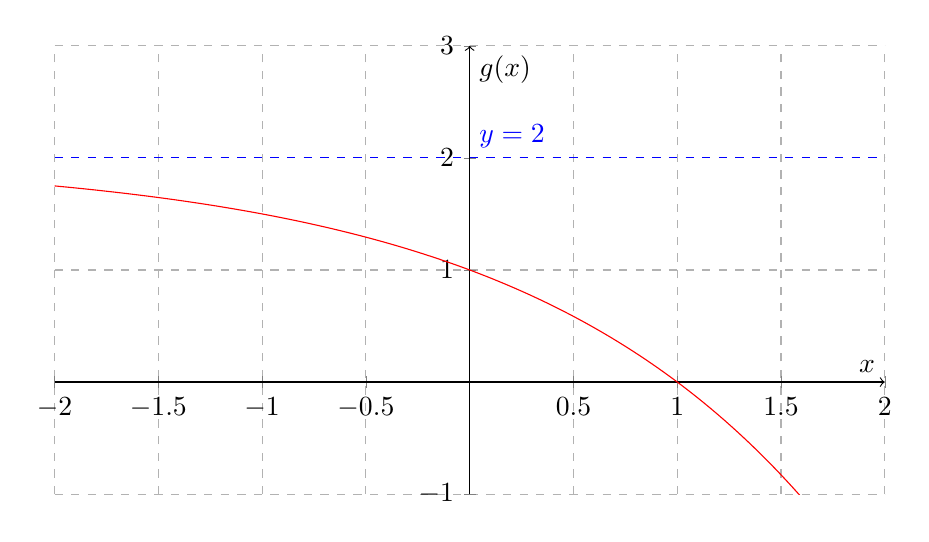
\begin{tikzpicture}
            \begin{axis}[
                xlabel=$x$,
                ylabel=$g(x)$,
                xmin=-2, xmax=2,
                ymin=-1, ymax=3,
                axis lines=middle,
                axis line style={->},
                legend style={at={(0.95,0.95)},anchor=north east},
                grid=both,
                major grid style={dashed,gray!60},
                width=\textwidth,
                height=0.6\textwidth,
                legend style={font=\small},
                legend cell align={left},
            ]

            % Function
            \addplot[red, domain=-2:2, samples=100, smooth] {-2^x + 2};

            % Asymptote
            \draw[dashed, blue] (axis cs:-2,2) -- (axis cs:2,2) node[midway,above right,blue]{$y=2$};

            \end{axis}
        \end{tikzpicture}
    \end{minipage}
   \vspace{0.5cm}
   
   $\{y \in \mathbb{R} \mid y < 2\}$   
\end{enumerate}
\end{example}

\newpage 
\begin{example}
    Ex.1: For the function, find:
        \begin{enumerate}
            \item Parent function 
            \item Horiz asymptote
            \item y-int
            \item Transformations
            \item Domain \& Range 
        \end{enumerate}
    \begin{enumerate}[label=\alph*.]
    \item $f(x)= 4^{2(x+5)}-8$ \\
    Parent function: $4^x$ \\
    Transformation: 
    \begin{enumerate}
        \item HS by $\frac{1}{2}$
        \item HT 5 $\gets$
        \item VT 8 $\downarrow$
    \end{enumerate}
    y-int:
    \begin{align*}
        f(0) & = 4^{2(0+5)}-8 \\
        & = 4^{10}-8 \\
        & = 1048568
    \end{align*}
    H.A: $ y= -8$ \\ 
    Domain: $\{x \in \mathbb{R}\}$
    Range:  $\{y \in \mathbb{R} \mid y > -8\}$
    \end{enumerate}
\end{example}

\newpage 
\begin{lesson}{Graphing Exponential Functions}
\underline{Ex.1}: The function \(y=3^x\) is an exponential function because the exponent is a variable.\\

Now, let's look at how to graph the exponential function \(y=3^x\).

\begin{table}[h]
    \centering
    \begin{minipage}{0.5\linewidth}
        \centering
    \begin{tabular}{|c|c|c|c|}
    \hline
    $x$ & $y=3^x$ & $y$ & $(x,y)$ \\
    \hline
    $-3$ & $3^{-3} = \frac{1}{3^3}$ & $\frac{1}{27}$ & $(-3, \frac{1}{27})$ \\
    $-2$ & $3^{-2} = \frac{1}{3^2}$ & $\frac{1}{9}$ & $(-2, \frac{1}{9})$ \\
    $-1$ & $3^{-1} = \frac{1}{3^1}$ & $\frac{1}{3}$ & $(-1, \frac{1}{3})$ \\
    $0$ & $3^0 = 1$ & $1$ & $(0, 1)$ \\
    $1$ & $3^1 = 3$ & $3$ & $(1, 3)$ \\
    $2$ & $3^2 = 9$ & $9$ & $(2, 9)$ \\
    $3$ & $3^3 = 27$ & $27$ & $(3, 27)$ \\
    \hline 
    \end{tabular}

    \end{minipage}%
    \begin{minipage}{0.5\linewidth}
        \centering
        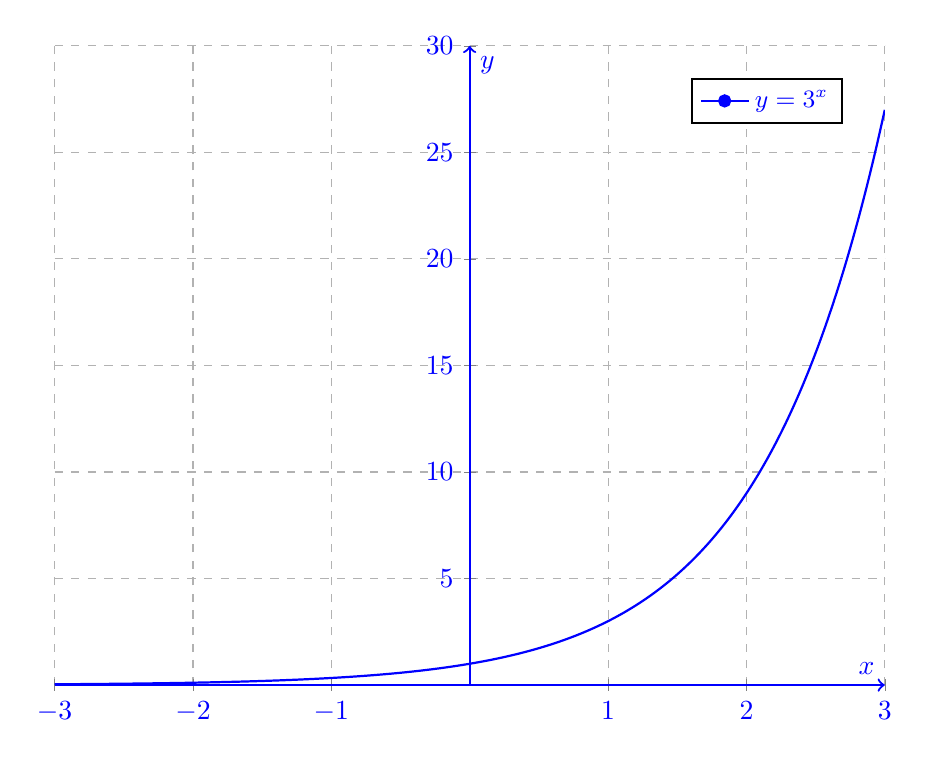
\begin{tikzpicture}
            \begin{axis}[
                xlabel=$x$,
                ylabel=$y$,
                xmin=-3, xmax=3,
                ymin=0, ymax=30,
                axis lines=middle,
                axis line style={->},
                legend style={at={(0.95,0.95)},anchor=north east},
                grid=both,
                major grid style={dashed,gray!60},
                width=\linewidth,
                height=0.8\textwidth,
                legend style={font=\small},
                legend cell align={left},
                domain=-3:3,
                samples=100,
                smooth,
                blue,
                thick,
                mark=*,
                mark options={blue,fill=blue}
            ]
            
            % Plot y=3^x
            \addplot[blue] {3^x};
            \addlegendentry{$y = 3^x$}
            
            \end{axis}
        \end{tikzpicture}
    \end{minipage}
\end{table}
\textbf{\underline{Definition 1}}: Since the y values increase as the x values increase in the example above, this is what we call exponential \textbf{\textcolor{blue}{Growth}}. (The graph goes up the hill from left to right) \\ \\
\textbf{\underline{QUESTION}}: In the exponential function \(y=3^x\), the y=values can never equal or be less than \textbf{\underline{zero}}. \\ \\ 

\textbf{\underline{Definition 2}}: Since the y-values can NEVER equal to zero in this function, there is a horizontal \underline{asymptote} at \(y=0\). \\ \\ 

\underline{\textbf{Ex.2}}: By looking at the graph above, list the domain and range of the function \(y=3^x\).\\

\textbf{Domain}:$\{x \in \mathbb{R}\}$. This is because the function is defined for every real value of \(x\). \\

\textbf{Range}: $\{y \in \mathbb{R} \mid y > 0\}$. This is evident from the graph, where the values of \(y\) are positive for all corresponding values of \(x\). \\ \\ 
\end{lesson}
\underline{\textbf{Ex.3}}: Consider the function \(y=\left(\frac{1}{3}\right)^x\). Analyze the graph and determine its domain and range.\\

\begin{table}[h]
    \centering
    \begin{minipage}{0.5\linewidth}
        \centering
        \begin{tabular}{|c|c|c|c|}
            \hline
            $x$ & $y=\left(\frac{1}{3}\right)^x$ & $y$ & $(x,y)$ \\
            \hline
            $-3$ & $27$ & $27$ & $(-3, 27)$ \\
            $-2$ & $9$ & $9$ & $(-2, 9)$ \\
            $-1$ & $3$ & $3$ & $(-1, 3)$ \\
            $0$ & $1$ & $1$ & $(0, 1)$ \\
            $1$ & $\frac{1}{3}$ & $\frac{1}{3}$ & $(1, \frac{1}{3})$ \\
            $2$ & $\frac{1}{9}$ & $\frac{1}{9}$ & $(2, \frac{1}{9})$ \\
            $3$ & $\frac{1}{27}$ & $\frac{1}{27}$ & $(3, \frac{1}{27})$ \\
            \hline 
        \end{tabular}
    \end{minipage}%
    \begin{minipage}{0.5\linewidth}
        \centering
        \begin{tikzpicture}
            \begin{axis}[
                xlabel=$x$,
                ylabel=$y$,
                xmin=-3, xmax=3,
                ymin=0, ymax=1,
                axis lines=middle,
                axis line style={->},
                legend style={at={(0.95,0.95)},anchor=north east},
                grid=both,
                major grid style={dashed,gray!60},
                width=\linewidth,
                height=0.8\textwidth,
                legend style={font=\small},
                legend cell align={left},
                domain=-3:3,
                samples=100,
                smooth,
                blue,
                thick,
                mark=*,
                mark options={blue,fill=blue}
            ]
            
            % Plot y=(1/3)^x
            \addplot[blue] {(1/3)^x};
            \addlegendentry{$y = \left(\frac{1}{3}\right)^x$}
            
            \end{axis}
        \end{tikzpicture}
    \end{minipage}
\end{table}
\textbf{\underline{Definition 2}}: Since the y-values decrease as the x-values increase in the example above, this is what we call exponential \textcolor{blue}{decay}. (The graph goes down the hill from left to right). \\ \\ 
\textbf{\underline{QUESTION}}: Is there an asymptote? If so, where it is? \\  \\
Yes , it is on "y=0".\\ \\
\underline{\textbf{Ex.4}}: By looking at the graph above, list the domain and range of the function \(y=(\frac{1}{3})^x\).\\ \\

\textbf{Domain}:$\{x \in \mathbb{R}\}$. This is because the function is defined for every real value of \(x\). \\

\textbf{Range}: $\{y \in \mathbb{R} \mid y > 0\}$. This is evident from the graph, where the values of \(y\) are positive for all corresponding values of \(x\). \\ \\ 
\underline{\textbf{Ex.3}}: Consider the function \(y=\left(\frac{1}{3}\right)^x\). Analyze the graph and determine its domain and range.\\
\begin{lesson}{1 - Exponential Growth}
\textcolor{blue}{Exponential growth} is a captivating concept where a quantity increases at a fixed percentage rate over time. This growth is modeled by the formula $y = ab^x$, where $a$ is the initial amount, $b$ is the growth factor, and $x$ is the time variable.

\begin{example}
Suppose you invest $1000$ at an annual interest rate of $5\%$, compounded annually. The growth formula is $A = 1000 \times (1 + 0.05)^x$. After 3 years, the amount would be approximately $A = 1000 \times (1 + 0.05)^3 \approx 1157.63$.
\end{example}

\begin{note}
The graph of an exponential growth function is characterized by a distinct upward curve that becomes steeper as $b$ increases.

\begin{center}
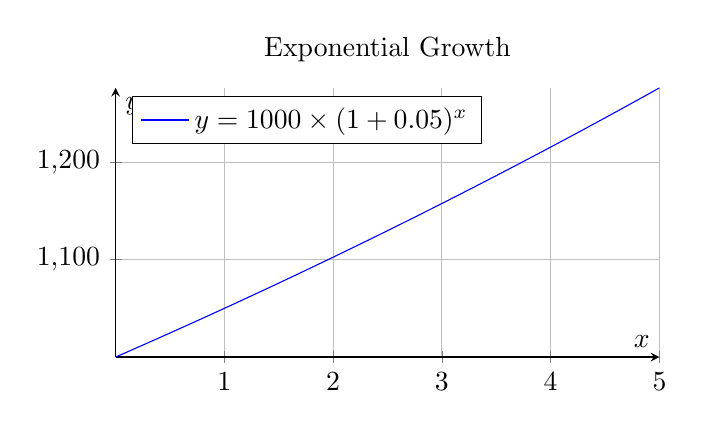
\begin{tikzpicture}
\begin{axis}[
  xlabel=$x$,
  ylabel=$y$,
  grid=major,
  axis lines=middle,
  width=0.7\linewidth,
  height=5cm,
  title={Exponential Growth},
  legend pos=north west,
]
\addplot[blue, domain=0:5, samples=100, smooth] {1000 * (1 + 0.05)^x};
\addlegendentry{$y = 1000 \times (1 + 0.05)^x$}
\end{axis}
\end{tikzpicture}
\end{center}
\end{note}
\end{lesson}
\newpage
\begin{lesson}{2 - Exponential Decay}
\textcolor{blue}{Exponential decay} is the counterpart to exponential growth. It occurs when a quantity decreases at a fixed percentage rate over time. The decay is modeled by the formula $y = ab^x$, where $b$ is between 0 and 1.

\begin{example}
Consider a radioactive substance that decays at a rate of 10\% per year. Its decay formula is $N = N_0 \times 0.9^t$. After 5 years, the remaining quantity is $N = N_0 \times 0.9^5$.
\end{example}

\begin{note}
The graph of an exponential decay function exhibits a decreasing curve that approaches but never reaches zero.

\begin{center}
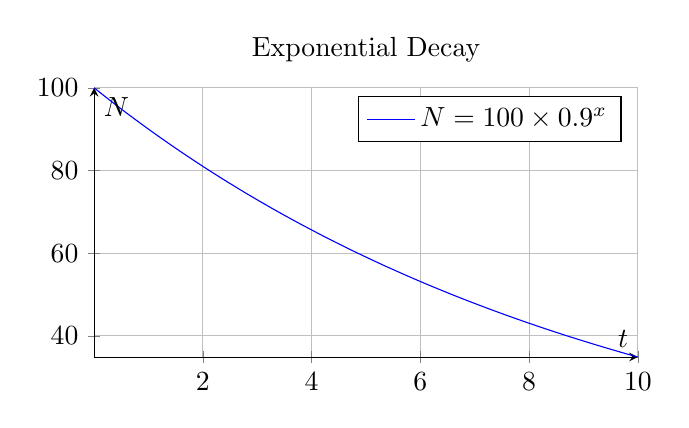
\begin{tikzpicture}
\begin{axis}[
  xlabel=$t$,
  ylabel=$N$,
  grid=major,
  axis lines=middle,
  width=0.7\linewidth,
  height=5cm,
  title={Exponential Decay},
  legend pos=north east,
]
\addplot[blue, domain=0:10, samples=100, smooth] {100 * 0.9^x};
\addlegendentry{$N = 100 \times 0.9^x$}
\end{axis}
\end{tikzpicture}
\end{center}
\end{note}
\end{lesson}
\newpage
\begin{lesson}{3 - Compound Interest}
\textcolor{blue}{Compound interest} is a powerful concept where interest is added to the initial principal, which then earns interest over time. The compound interest formula is given by $A = P(1 + r/n)^{nt}$, where $A$ is the final amount, $P$ is the principal, $r$ is the annual interest rate, $n$ is the number of times interest is compounded per year, and $t$ is the time in years.

\begin{example}
Imagine investing $5000$ at an annual interest rate of $6\%$, compounded quarterly. The formula is $A = 5000 \times (1 + 0.06/4)^{4t}$. After 2 years, the amount is $A = 5000 \times (1 + 0.06/4)^{4 \times 2}$.
\end{example}

\begin{note}
Compound interest enables your investment to grow faster compared to simple interest, especially with more frequent compounding.
\end{note}
\end{lesson}
\newpage 
\begin{lesson}{4 - Properties of Exponential Functions}
\textcolor{blue}{Exponential functions} possess several key properties:

\begin{itemize}
    \item They have a constant base.
    \item They can model growth or decay.
    \item They have an asymptote, which they approach but never reach.
    \item They are always positive if the base is greater than 1.
    \item They are always decreasing if the base is between 0 and 1.
\end{itemize}

\begin{example}
Consider the function $f(x) = 2^x$. It has a constant base of 2 and models exponential growth.
\end{example}

\begin{note}
The graph of an exponential function approaches but never crosses the horizontal axis (asymptote).

\begin{center}
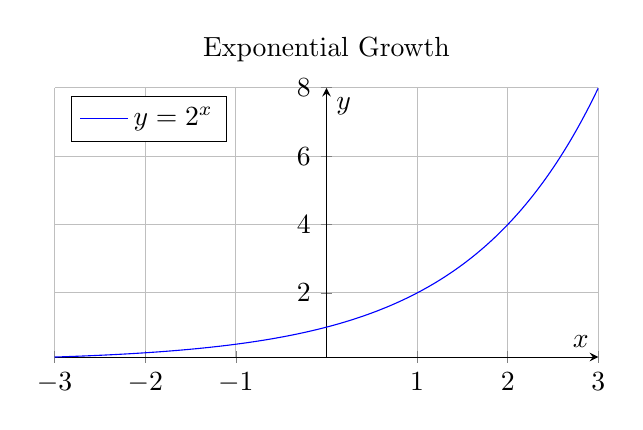
\begin{tikzpicture}
\begin{axis}[
  xlabel=$x$,
  ylabel=$y$,
  grid=major,
  axis lines=middle,
  width=0.7\linewidth,
  height=5cm,
  title={Exponential Growth},
  legend pos=north west,
]
\addplot[blue, domain=-3:3, samples=100, smooth] {2^x};
\addlegendentry{$y = 2^x$}
\end{axis}
\end{tikzpicture}
\end{center}
\end{note}
\end{lesson}
\newpage 
\begin{lesson}{5 - Transformations}
\textcolor{blue}{Transformations} offer a way to modify the graph of an exponential function. Common transformations include vertical shifts, horizontal shifts, reflections, and stretches or compressions. These transformations are applied to the base function $y = b^x$.

\begin{example}
If $g(x) = 3 \times 2^x$, the function $g$ is a vertical stretch of $f(x) = 2^x$ by a factor of 3.
\end{example}

\begin{note}
Transformations alter the appearance and behavior of the exponential function graph.

\begin{center}
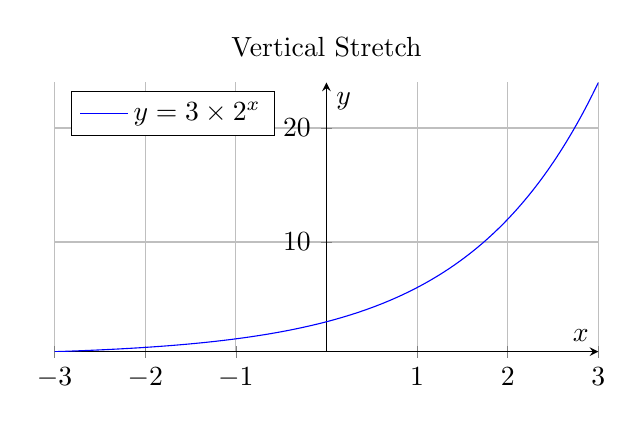
\begin{tikzpicture}
\begin{axis}[
  xlabel=$x$,
  ylabel=$y$,
  grid=major,
  axis lines=middle,
  width=0.7\linewidth,
  height=5cm,
  title={Vertical Stretch},
  legend pos=north west,
]
\addplot[blue, domain=-3:3, samples=100, smooth] {3 * 2^x};
\addlegendentry{$y = 3 \times 2^x$}
\end{axis}
\end{tikzpicture}
\end{center}
Transformations can also involve horizontal shifts, reflections, and other modifications to customize the behavior of the exponential function graph.
\end{note}
\end{lesson}



\newpage
\begin{lesson}{6 - Applications of Exponential Functions}
\begin{center}
\begin{minipage}{0.4\textwidth}
\begin{equation*}
    A = P(1+i)^n
\end{equation*}
\end{minipage}%
\begin{minipage}{0.6\textwidth}
Where:
\begin{itemize}
    \item A is the final amount
    \item P is the initial amount 
    \item i is the growth/decay rate
    \item n is the total number of growth/decay periods
\end{itemize}
\end{minipage}
\end{center}
Doubling Times: An increase of 100\% (or 1) which makes the base equal to 2. \\ \\
$$A = P(1+i)^n$$ 
$$\therefore A = P(2)^n$$
Half-Lives: A decrease of 50\%(or 0.5) which makes the base equal to $\frac{1}{2}$.
$$A=P(1-0.5)^n$$
$$\therefore A = P(0.5)$$
or
$$A = P(\frac{1}{2})^n$$
\end{lesson}
\begin{example}
    1.The element Duzzanium has a half-life of 4 months. If there are 5000 g of Duzzanium today, how much will there be in 2 years?
\end{example}
\begin{example}
    2. A bacterial culture began with 7500 bacteria. It's growth can be modeled using the formula $N=7500(2)^{\frac{t}{36}}$, where N is the number of bacteria after t hours.
\begin{enumerate}[label=\alph*.]
    \item What is the doubling time of the bacteria?
    \item How many bacteria are present after 36 hours?
    \item How many bacteria are present after 3 days?
    \item Approximately how many hours will pass for the culture to reach 2 million bacteria?
\end{enumerate}
    
\end{example}
\newpage

\newpage
\begin{lesson}{ Summative Assessment }
\begin{enumerate}
    \item \textbf{Evaluate the following:}
    \begin{enumerate}[label=\alph*)]
        \item $2^3$:
        \begin{align*}
            2^3 &= 2 \times 2 \times 2 \\
            &= 8
        \end{align*}
        
        \item $10^{-2}$:
        \begin{align*}
            10^{-2} &= \frac{1}{10^2} \\
            &= \frac{1}{100} \\
            &= 0.01
        \end{align*}
        
        \item $e^0$:
        \begin{align*}
            e^0 &= 1
        \end{align*}
    \end{enumerate}
    
    \item \textbf{Solve for $x$:}
    \begin{enumerate}[label=\alph*)]
        \item $5^x = 125$:
        \begin{align*}
            5^x &= 125 \\
            x &= 3
        \end{align*}
        
        \item $2e^{2x} = 16$:
        \begin{align*}
            e^{2x} &= 8 \\
            2x &= \ln(8) \\
            x &= \frac{\ln(8)}{2}
        \end{align*}
    \end{enumerate}
\newpage
    \item \textbf{Consider the function $f(x) = 3 \times 2^x$. Perform the following transformations and sketch the resulting graph:}
    \begin{enumerate}[label=\alph*)]
        \item \textbf{Vertical stretch by a factor of 2:}
        The function becomes $g(x) = 6 \times 2^x$.
        
        \item \textbf{Horizontal shift right by 1 unit:}
        The function becomes $h(x) = 3 \times 2^{(x - 1)}$.
        
        \item \textbf{Reflection across the $x$-axis:}
        The function becomes $k(x) = -3 \times 2^x$.
        
        \textbf{Graph:} (Note: This is a conceptual sketch; precise plotting requires numerical values.)

\definecolor{lessonbgcolor}{rgb}{0.9,0.9,1}
\definecolor{examplecolor}{rgb}{0.8,1,0.8}
\definecolor{blue}{RGB}{0,70,170}

\pgfplotsset{
    compat=1.17,
    every axis/.append style={
        axis line style={->},
        xlabel style={anchor=west},
        ylabel style={anchor=south},
        legend style={at={(0.03,0.97)}, anchor=north west, draw=none, fill=none, font=\scriptsize},
    },
}


\begin{figure}[h]
    \centering
    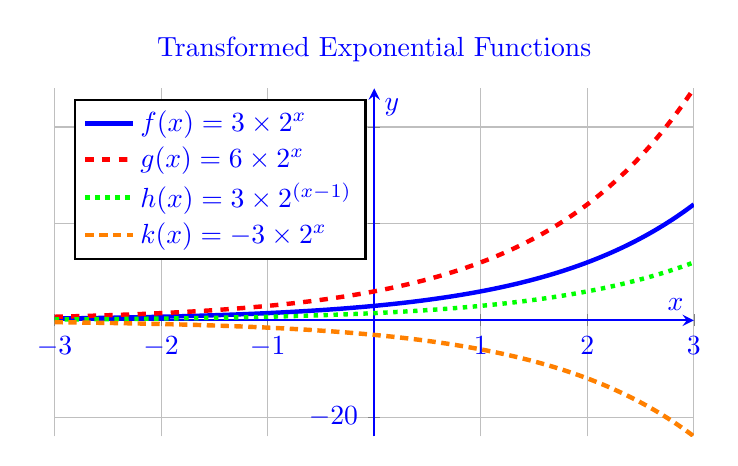
\begin{tikzpicture}
        \begin{axis}[
            xlabel={$x$},
            ylabel={$y$},
            grid=major,
            axis lines=middle,
            width=0.8\linewidth,
            height=6cm,
            title={Transformed Exponential Functions},
            legend pos=north west,
            domain=-3:3,
            samples=100,
            smooth,
            blue,
            thick,
            every axis plot/.append style={ultra thick},
            legend cell align=left,
        ]
            \addplot [blue] {3 * 2^x};
            \addlegendentry{$f(x) = 3 \times 2^x$}
            
            \addplot [red, dashed] {6 * 2^x};
            \addlegendentry{$g(x) = 6 \times 2^x$}
            
            \addplot [green, dotted] {3 * 2^(x - 1)};
            \addlegendentry{$h(x) = 3 \times 2^{(x - 1)}$}
            
            \addplot [orange, densely dashed] {-3 * 2^x};
            \addlegendentry{$k(x) = -3 \times 2^x$}
        \end{axis}
    \end{tikzpicture}
    \caption{Transformed Exponential Functions}
    \label{fig:transformed-exponential}
\end{figure}
    \end{enumerate}
\end{enumerate}
\end{lesson}
\begin{note}
    When considering the function \(y=a^x\):

    \textbf{Exponential Growth:} If $a > 1$, the function exhibits exponential growth. In this case, as $x$ increases, the corresponding values of $y$ grow rapidly.

    \textbf{Exponential Decay:} If $0 < a < 1$, the function demonstrates exponential decay. In such instances, as $x$ increases, the values of $y$ diminish rapidly, showcasing a decay behavior.
\end{note}
\end{document}
